\section{Background}
This section provides a high level description of the pieces of the puzzle necessary in order to understand our approach. We describe the relevant algorithms and tools in order to make the later formalisms fit into the full picture. 

\subsection{Inductive Validity Cores}

Given a complex model, it is often useful to extract traceability information related to the proof, in other words, which portions of the model were necessary to construct the proof. An algorithm was introduced by Ghassabani, et. al. to provide Inductive Validity Cores (IVCs) as a way to determine which model elements are necessary for the inductive proofs of the safety properties for sequential systems~\cite{GhassabaniGW16}. Given a safety property of the system, a model checker can be invoked in order to construct a proof of the property. The IVC generation algorithm can extract traceability information from that proof process and return a minimal set of the model elements required in order to prove the property. A short time later, this algorithm was refined in order to produce all such minimal sets of IVC elements~\cite{Ghassabani2017EfficientGO}. 

This algorithm is of interest to us for the following reason. By letting the negation of the safety property of interest be our top level event, we can utilize the algorithm to find the set of minimal IVCs which will tell us the minimal model elements (including faults) necessary to prove that this top level event occurs. In other words, we will know the minimal set of events required in order to cause the occurance of the top level event. These model elements consist of the active faults present in the system and the contracts of components that were effected by the presence of the fault. This gives a trace of how the fault propagates through system components and how the software behaves in the presence of the faults. 

In section III, we show the formal definitions of IVCs in detail. \\

Our approach utilizes a few tools in order to generate the artifacts of interest and a brief background will be helpful. and hence the rest of the background section consists of a brief description of AADL, AGREE, and the SOTERIA tools and languages. 

\subsection{Architecture Analysis and Design Language}
We are using the Architectural Analysis and Design Language (AADL) to construct system architecture models.  AADL is an SAE International standard that defines a language and provides a unifying framework for describing the system architecture for ``performance-critical, embedded, real-time systems''~\cite{AADL_Standard,FeilerModelBasedEngineering2012}. From its conception, AADL has been designed for the design and construction of avionics systems.  Rather than being merely descriptive, AADL models can be made specific enough to support system-level code generation.  Thus, results from analyses conducted, including the new safety analysis proposed here, correspond to the system that will be built from the model.  

An AADL model describes a system in terms of a hierarchy of components and their interconnections, where each component can either represent a logical entity (e.g., application software functions, data) or a physical entity (e.g., buses, processors). An AADL model can be extended with language annexes to provide a richer set of modeling elements for various system design and analysis needs (e.g., performance-related characteristics, configuration settings, dynamic behaviors). The language definition is sufficiently rigorous to support formal analysis tools that allow for early phase error/fault detection.

\subsection{Compositional Analysis} Compositional analysis of systems was introduced in order to address the scalability of model checking large software systems. Monolithic verification and compositional verification are two ways that mathematical verification of component properties can be performed. In monolithic analysis, the model is flattened and the top level properties are proved using only the leaf level contracts of the components. On the other hand, the analysis can be performed compositionally following the architecture hierarchy such that analysis at a higher level is based on the components at the next lower level. The idea is to partition the formal analysis of a system architecture into verification tasks that correspond into the decomposition of the architecture. A component contract is an assume-guarantee pair. Intuitively, the meaning of a pair is: if the assumption is true, then the component will ensure that the guarantee is true. The components of a system are organized hierarchically and the proofs begin at the leaf level. Each layer of the architecture is viewed a system. For any given layer, the proof consists of demonstrating that the system guarantee is provable given the behavior of its subcomponents and the system assumptions. This proof is performed one layer at a time from the leaf level up to the top level of the system. When compared to monolithic analysis (i.e., analysis of the flattened model composed of all components), the compositional approach allows the analysis to scale to much larger systems~\cite{NFM2012:CoGaMiWhLaLu}. 

\subsection{Assume Guarantee Reasoning Environment}
The Assume Guarantee Reasoning Environment (AGREE) is a tool for formal analysis of behaviors in AADL models~\cite{NFM2012:CoGaMiWhLaLu}.  It is implemented as an AADL annex and annotates AADL components with formal behavioral contracts. Each component's contracts can include assumptions and guarantees about the component's inputs and outputs respectively, as well as predicates describing how the state of the component evolves over time.

AGREE translates an AADL model and the behavioral contracts into Lustre~\cite{Halbwachs91:IEEE} and then queries a user-selected
model checker to conduct the back-end analysis. The analysis can be performed compositionally or monolithically.

\subsection{Safety Annex for AADL}
The Safety Annex for AADL is a tool that provides the ability to reason about faults and faulty component behaviors in AADL models~\cite{Stewart17:IMBSA,SATechReport}. In the Safety Annex approach, formal assume-guarantee contracts are used to define the nominal behavior of system components. The nominal model is verified using AGREE. The Safety Annex weaves faults into the nominal model and analyzes the behavior of the system in the presence of faults. The tool supports behavioral specification of faults and their implicit propagation through behavioral relationships in the model as well as provides support to capture binding relationships between hardware and software compönents of the system. 

\subsection{SOTERIA}
The Safe and Optimal Techniques Enabling Recovery, Integrity, and Assurance (SOTERIA) tool is used to perform safety analysis of Integrated Modular Avionics (IMA) systems~\cite{SOTERIAproject}. In the SOTERIA project, a compositional modeling language was developed and this language is used as input in order to automatically synthesize the qualitative and quantitative safety analyses. The tool is compositional in that it requires safety aspects at each component level which enables the generation of compositional fault trees. 

\begin{figure}[h]
\begin{center}
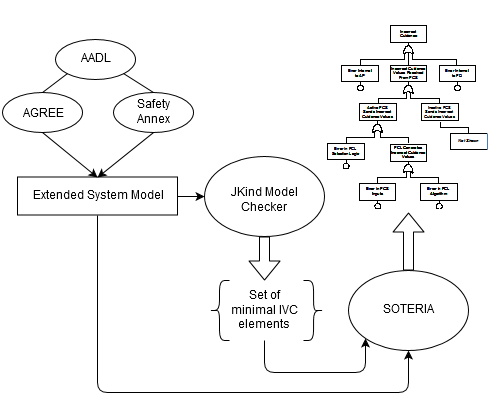
\includegraphics[width=8cm]{images/processFTA.png}
\caption{Outline of the fault tree generation process} \label{fig:processFTA}
\end{center}
\end{figure}

\subsection{Fault Tree Analysis} A Fault Tree (FT) is a directed acyclic graph whose leaves model component failures and whose gates model failure propagation. The system failure under examination is the root of the tree and is called the Top Level Event (TLE). The node types in a fault tree are \textit{events} and \textit{gates}. An event is an occurance within the system, typically the failure of a subsystem down to an individual component. Events can be grouped into Basic Events (BEs), which occur independently, and \textit{intermediate events} which occur dependently and are caused by one or more other events.  These events model the failure of the system (or subsystem) under consideration. The gates represent how failures propagate through the system and how failures in subsystems can cause system wide failures. The two main logic symbols used are the Boolean logic AND-gates and OR-gates. An AND-gate is used when the undesired top level event can only occur when all the lower conditions are true. The OR-gate is used when the undesired event can occur if any one or more of the next lower conditions is true. This is not a comprehensive list of gate types, but we focus our attention on these two common gate types. 

Figure~\ref{fig:introFT} shows a simple example of a fault tree based on SAE ARP4761~\cite{SAE:ARP4761}. In this example, the top level event corresponds to an aircraft losing all wheel braking. In order for this event to occur, all of the basic events must occur. This is seen through the use of the AND gate below the top level event. The gates in the fault tree describe how failures propagate through the system. Each gate has one output and one or more inputs. In Figure~\ref{fig:introFT}, the AND gate has three inputs and one output. The leaves of the tree represent the basic events of the system and in the case of this fault tree, these three events are also the Minimum Cut Set (MCS) for this top level event. An MCS is the minimum set of basic events that must occur together in order to cause the TLE to occur. Finding these sets is important to FTA and has been an active area of interest in the research community since fault trees were first described in Bell Labs in 1961~\cite{historyFTA,0f356f05e72f43018211b36f97c8854a}. 

\begin{figure}[h]
\begin{center}
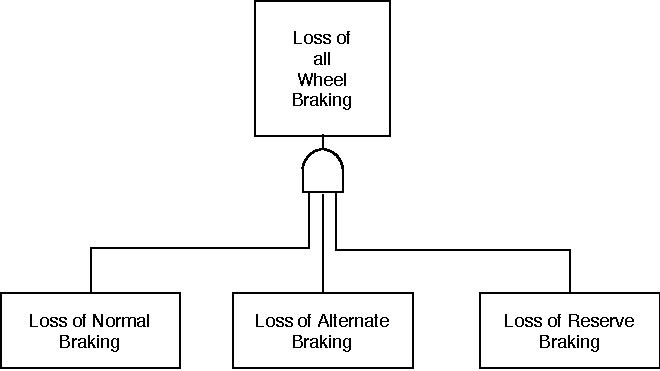
\includegraphics[width=8cm]{images/introFT2.pdf}
\caption{A simple fault tree} \label{fig:introFT}
\end{center}
\end{figure}

There are two main types of FTA that we differentiate here as \textit{qualitative} analysis and \textit{quantitative} analysis. In qualitative analysis, the structure of the fault tree is considered and the cut sets are a way to indicate which combinations of component failures will cause the system to fail. On the other hand, in quantitative analysis the probability of the TLE is calculated given the probability of occurance of the basic events. 

The formal definition of a fault tree is provided in section III and more details regarding quantitative and qualitative FTA is explained there as well. 

The general outline of our process is as follows and is shown in Figure~\ref{fig:processFTA}. The AADL system model is annotated with behavioral contracts using AGREE and then extended with faults using the Safety Annex. This combination of the system model (AADL), component contracts (AGREE), and fault definitions (Safety Annex) comprise the extended system model as shown in the figure. During the analysis of the extended system model, a customized Lustre program is generated for each layer of the architecture and this is fed to JKind model checker~\cite{2017arXiv171201222G}. JKind has the ability to do online enumeration of the sets of elements required in order to prove the properties at the current level of analysis, these are called Inductive Validity Cores (IVCs). Once these elements are collected, we know the minimal set of model elements required in order to prove the top level property. When this property is stated as a top level event, this gives us our minimal cut sets required in order to generate a fault tree. These IVC elements and pertinant details of the extended system model is given to the SOTERIA tool whose output is the graphical fault tree representation of the input. 

